\documentclass{beamer}

\mode<presentation>
{
  \usetheme{RT}
  \setbeamercovered{transparent}
  \usecolortheme{RT}
}
\usefonttheme{professionalfonts} 	% optional

\setbeamertemplate{footline}[frame number]{}


 %%######## Choose LANGUAGE

 %%% English
    \usepackage[english]{babel}		% comment if cause of errors
    \selectlanguage{english}		% (due to MikTex - babel versions)

 %%% German
%    \usepackage[english,ngerman]{babel}
%    \selectlanguage{ngerman}
   % %% In some cases you might need that
   % \usepackage{german}
    \usepackage[latin1]{inputenc}
    
% math environments and more by the AMS 
\PassOptionsToPackage{fleqn}{amsmath}		
 \usepackage{amsmath}

%When using tikZ one must also use the color package.
\PassOptionsToPackage{usenames,dvipsnames}{color}
 \usepackage{color}
%This package lets you compile tikz graphics.
 \usepackage{tikz}
 \usepackage{pgfplots}
 \usetikzlibrary{decorations.markings}
 \usepackage{standalone}

%Code Listings
\usepackage{listings} 
\lstset{language=Matlab,
    keywordstyle=\color{blue},%\bfseries,
    basicstyle=\small\ttfamily,
    identifierstyle=\color{blue},
    %commentstyle=\color{green}\ttfamily,
    stringstyle=\rmfamily,
    numbers=none,%left,%
    numberstyle=\scriptsize,%\tiny
    stepnumber=5,
    numbersep=8pt,
    showstringspaces=false,
    breaklines=true,
    frameround=ftff,
    frame=single,
    belowcaptionskip=.75\baselineskip
    %frame=L
} 


 %%######## Chose FONT
\usepackage[T1]{fontenc}
% Note that the encoding and the font should match. If T1
% does not look nice, try deleting the line with the fontenc.

%\usepackage[utf8]{inputenc}
\usepackage{times}



 %%######## GRAPHICS Options
\graphicspath{{figures/}}				% Define the path to the figures

\usepackage{ifpdf}

\ifpdf % pdfTeX
	\DeclareGraphicsExtensions{.pdf,.png,.jpg,.gif,.pdftex}
	\DeclareGraphicsRule{.pdftex}{pdf}{*}{}	% for xfig exported files
	\newcommand{\xfig}[2]{\scalebox{#1}{\input{"../figures/#2.pdftex_t"}}} % XFIG
\else % DVI
	\DeclareGraphicsExtensions{.eps,.pstex}
	\DeclareGraphicsRule{.pstex}{eps}{*}{}		% for xfig exported files
	\newcommand{\xfig}[2]{\scalebox{#1}{\input{"../figures/#2.pstex_t"}}} % XFIG
	%\usepackage{psfrag}		% might be useful
\fi

 % Other figures (e.g., MATLAB  EPS or PDF figures)
\newcommand{\afig}[2]{\includegraphics[scale=#1]{#2}}

 % figures defined in TeX files
\newcommand{\tfig}[2]{\scalebox{#1}{\input{"#2.tex"}}}



 %%######## Logos only on Title page
\titlegraphic{\vspace{0.1cm}
\includegraphics[height=0.8cm]{../figures/kuLeuven.png} \hfill 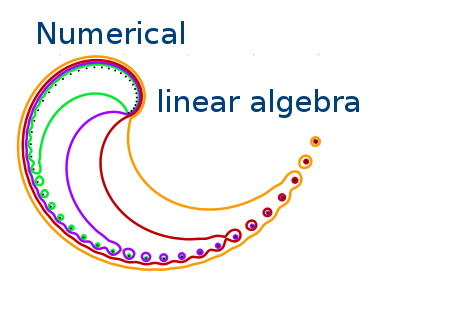
\includegraphics[height=1.9cm]{../figures/numLinLogo.png}}




 %%######## Other FUNCTIONS

\newcommand{\vs}[1]{\vspace{#1mm}}

\newcommand{\bbma} {\begin{bmatrix} }
\newcommand{\ebma} {\end{bmatrix}}

 % Some color definitions
\setbeamercolor{greenhead}{fg=white,bg=green!80!black}%
\setbeamercolor{greenbody}{fg=black,bg=green!50!white}%

\setbeamercolor{redhead}{fg=white,bg=red!80!black}%
\setbeamercolor{redbody}{fg=black,bg=red!50!white}%
